%%%%%%%%%%%%%%%%%%%%%%%%%%%%%%%%%%%%%%%%%
% Short Sectioned Assignment LaTeX Template Version 1.0 (5/5/12)
% This template has been downloaded from: http://www.LaTeXTemplates.com
% Original author:  Frits Wenneker (http://www.howtotex.com)
% License: CC BY-NC-SA 3.0 (http://creativecommons.org/licenses/by-nc-sa/3.0/)
%%%%%%%%%%%%%%%%%%%%%%%%%%%%%%%%%%%%%%%%%

%----------------------------------------------------------------------------------------
%	PACKAGES AND OTHER DOCUMENT CONFIGURATIONS
%----------------------------------------------------------------------------------------

\documentclass[paper=a4, fontsize=11pt]{scrartcl} % A4 paper and 11pt font size

% ---- Entrada y salida de texto -----

\usepackage[T1]{fontenc} % Use 8-bit encoding that has 256 glyphs
\usepackage[utf8]{inputenc}
%\usepackage{fourier} % Use the Adobe Utopia font for the document - comment this line to return to the LaTeX default

% ---- Idioma --------

\usepackage[spanish, es-tabla]{babel} % Selecciona el español para palabras introducidas automáticamente, p.ej. "septiembre" en la fecha y especifica que se use la palabra Tabla en vez de Cuadro

% ---- Otros paquetes ----

\usepackage{url} % ,href} %para incluir URLs e hipervínculos dentro del texto (aunque hay que instalar href)
\usepackage{amsmath,amsfonts,amsthm} % Math packages
%\usepackage{graphics,graphicx, floatrow} %para incluir imágenes y notas en las imágenes
\usepackage{graphics,graphicx, float} %para incluir imágenes y colocarlas

% Para hacer tablas comlejas
%\usepackage{multirow}
%\usepackage{threeparttable}

%\usepackage{sectsty} % Allows customizing section commands
%\allsectionsfont{\centering \normalfont\scshape} % Make all sections centered, the default font and small caps

\usepackage{fancyhdr} % Custom headers and footers
\pagestyle{fancyplain} % Makes all pages in the document conform to the custom headers and footers
\fancyhead{} % No page header - if you want one, create it in the same way as the footers below
\fancyfoot[L]{} % Empty left footer
\fancyfoot[C]{} % Empty center footer
\fancyfoot[R]{\thepage} % Page numbering for right footer
\renewcommand{\headrulewidth}{0pt} % Remove header underlines
\renewcommand{\footrulewidth}{0pt} % Remove footer underlines
\setlength{\headheight}{13.6pt} % Customize the height of the header

\numberwithin{equation}{section} % Number equations within sections (i.e. 1.1, 1.2, 2.1, 2.2 instead of 1, 2, 3, 4)
\numberwithin{figure}{section} % Number figures within sections (i.e. 1.1, 1.2, 2.1, 2.2 instead of 1, 2, 3, 4)
\numberwithin{table}{section} % Number tables within sections (i.e. 1.1, 1.2, 2.1, 2.2 instead of 1, 2, 3, 4)

\setlength\parindent{0pt} % Removes all indentation from paragraphs - comment this line for an assignment with lots of text

\newcommand{\horrule}[1]{\rule{\linewidth}{#1}} % Create horizontal rule command with 1 argument of height

%	TÍTULO Y DATOS DEL ALUMNO
%----------------------------------------------------------------------------------------

\title{	
	\normalfont \normalsize 
	\textsc{\textbf{Planificación y Gestión de Proyectos Informáticos (2018-2019)} \\ Máster Profesional de Ingeniería Informática \\ Universidad de Granada} \\ [25pt] % Your university, school and/or department name(s)
	\horrule{0.5pt} \\[0.4cm] % Thin top horizontal rule
	\huge Práctica A-II \\ % The assignment title
	\horrule{2pt} \\[0.5cm] % Thick bottom horizontal rule
}

\author{Alejandro Campoy Nieves \\ Luis Gallego Quero} % Nombre y apellidos y correo
\date{\normalsize\today} % Incluye la fecha actual

\usepackage[spanish, es-tabla]{babel}
\usepackage{hyperref} % Para añadir los hiperenlaces.
\hypersetup{
	colorlinks=true,
	linkcolor=blue,
	filecolor=magenta,      
	urlcolor=cyan,
}
\usepackage{graphicx}
\usepackage{amssymb, amsmath, amsbsy}
\usepackage{mathptmx}	
\usepackage{float}
\usepackage{booktabs}					%paquete para realización de tablas profesionales
\usepackage{eurosym}
%\usepackage[table]{xcolor}
%\definecolor{lightgray}{gray}{0.9}
\usepackage{xcolor}
\usepackage{colortbl}


%----------------------------------------------------------------------------------------
% DOCUMENTO
%----------------------------------------------------------------------------------------

\begin{document}
	\maketitle % Muestra el Título
	
	\newpage %inserta un salto de página
	
	\tableofcontents % para generar el índice de contenidos
	
	\listoffigures
	
	\listoftables	
	
	\newpage	
 
\section{Restricciones de negocio}


\begin{table}[H]
	\begin{center}
		\begin{tabular}{|l|l|l|}
			\hline 
			Restricción de negocio & Información & Comentarios \\ 
			\hline \hline
			Presupuesto & 118000 euros & Depende de varias subvenciones \\ \hline
			Plazo máximo proyecto & Hasta Junio & \\ \hline
			Cobertura mínima & Necesitamos darle más prioridad  & Gran cantidad de los fondos \\ 
			 & a la cobertura del laboratorio & proviene de éste  \\ \hline
			Marca de los dispositivos de red & Marcas hardware Juniper & Cisco no es válido\\ \hline
			Límite construcción de la red & De 2 meses & Migración de datos prevista \\ \hline
		\end{tabular}
		\caption{Tabla de Restricciones de negocio.}
		\label{tabla:tabla1}
	\end{center}
\end{table}

\section{Restricciones técnicas}

\begin{table}[H]
	\begin{center}
		\begin{tabular}{|l|l|l|}
			\hline 
			Restricción técnica & Información & Comentarios \\ 
			\hline \hline
			Cobertura de la red & Al menos, en las plantas 4, 6 y 7 & Sería conveniente extenderlo \\
			& & al resto del hospital \\ \hline
			Compatibilidad & Se busca que el proyecto sea compatible & \\ 
		    & con lo configurado anteriormente & \\ \hline
			Software libre &  & \\ \hline
			Instalación remota & Ordenadores se instalan cada semana & Los viernes a las 21:00 \\ \hline
			Muestras telepatología & Cada muestra pesa entre 2 y 4 GB & \\ \hline		
		\end{tabular}
		\caption{Restricciones técnicas.}
		\label{tabla:tabla2}
	\end{center}
\end{table}




\section{Tabla de caracterización de usuarios}

\begin{table}[H]
	\begin{center}
		\begin{tabular}{|l|l|l|l|}
			\hline 
			Nombre de la comunidad de & Nombre de & Localización & Aplicaciones usadas \\
		    usuarios & miembros & & \\ 
			\hline \hline
			Recepcionista & & Recepción  & \\ \hline
			Directora & Aurora & Despacho de dirección  & \\ \hline
			 & 1 persona, & Servicio de informática & \\ 
			 & sin nombre & & \\ \hline
		    Secretaría & 2 personas,  & &  \\ 
		     & sin nombre & & \\ \hline
		    Centro de datos & 1 persona, & Centro de datos &  \\ 
		     & sin nombre & & \\ \hline
		    Séptima planta, sala de espera & Arturo  & Consultas &  \\ \hline
		    Cuarta planta, consultas & 1 persona, & Consultas planta cuarta & Historial clínico  \\ 
		    & sin nombre & & \\ \hline
		    Primera sala de telepatología & 1 persona, & Sala 1 telepatología & QuPath \\
		    & sin nombre & & \\ \hline
		\end{tabular}
		\caption{Tabla de caracterización de usuarios.}
		\label{tabla:tabla5}
	\end{center}
\end{table}

\section{Mapa}

\begin{figure}[h]
	\centering
		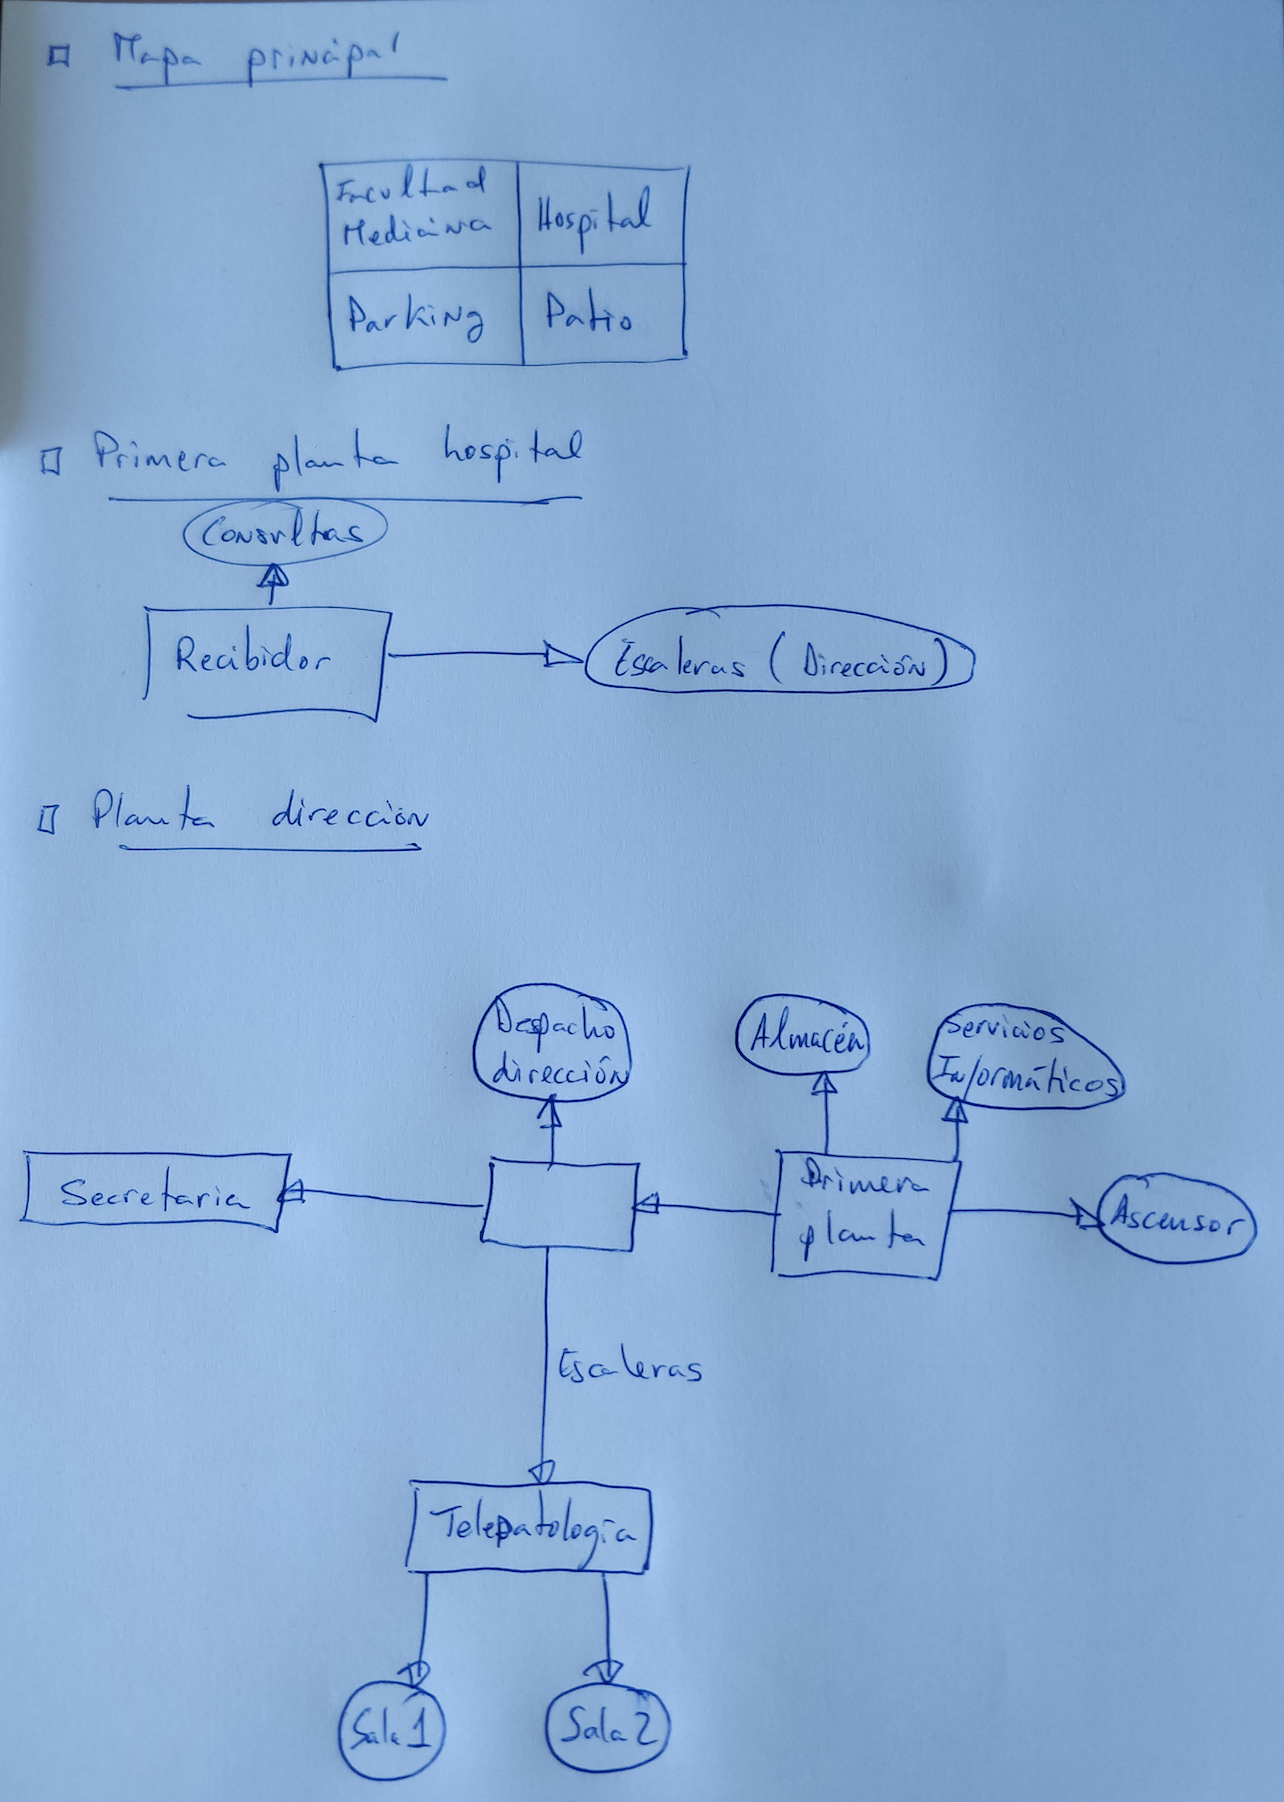
\includegraphics[scale=0.7]{./mapa.png}
	\caption{Mapa}
\end{figure}

%\newpage
%\bibliographystyle{plain}
%\bibliography{biblio}

\end{document}       
%---------------------------------------------------
